\section{Technologies Used}
		\vs
		\subsection{Server Side Technology}
		\begin{wrapfigure}{T}{0.3\textwidth}
			\centering
			\vspace{-60pt}
			
\includegraphics[width=0.25\textwidth]{nodejs.png}
			\vspace{-80pt}
		\end{wrapfigure}
		\vs
		\textbf{\Large node.js}
		\vs
		Node.js is an open-source, cross-platform, JavaScript runtime environment (Framework) that executes JavaScript code outside a web browser. Node.js lets developers use JavaScript to write command line tools and for server-side scripting—running scripts server-side to produce dynamic web page content before the page is sent to the user's web browser. Consequently, Node.js represents a "JavaScript everywhere" paradigm, unifying web-application development around a single programming language, rather than different languages for server- and client-side scripts.
		\vs
		Though .js is the standard filename extension for JavaScript code, the name "Node.js" doesn't refer to a particular file in this context and is merely the name of the product. Node.js has an event-driven architecture capable of asynchronous I/O. These design choices aim to optimize throughput and scalability in web applications with many input/output operations, as well as for real-time Web applications (e.g., real-time communication programs and browser games).

		\vs[1]
		\begin{wrapfigure}{T}{0.3\textwidth}
			\centering
			\vspace{-50pt}
			
\includegraphics[width=0.25\textwidth]{express.png}
			\vspace{-80pt}
		\end{wrapfigure}
		\vs
		\textbf{\Large express.js}
		\vs
	ExpressJS is a web application framework that provides you with a simple API to build websites, web apps and back ends. With ExpressJS, you need not worry about low level protocols, processes, etc.
	\vs
	Express provides a minimal interface to build our applications. It provides us the tools that are required to build our app. It is flexible as there are numerous modules available on npm, which can be directly plugged into Express.
	
	Express was developed by \textbf{TJ Holowaychuk} and is maintained by the Node.js foundation and numerous open source contributors.
	\vs[1]
	\begin{wrapfigure}{T}{0.3\textwidth}
		\centering
		\vspace{-30pt}
		
\includegraphics[width=0.25\textwidth]{mongo.png}
		\vspace{-80pt}
	\end{wrapfigure}
	\vs
	\textbf{\Large mongoDB}
	\vs
	MongoDB is a document-oriented NoSQL database used for high volume data storage. Instead of using tables and rows as in the traditional relational databases, MongoDB makes use of collections and documents. Documents consist of key-value pairs which are the basic unit of data in MongoDB. Collections contain sets of documents and function which is the equivalent of relational database tables. MongoDB is a database which came into light around the mid-2000s.
	\vs
	\textbf{\large Feature Of MongoDB}
	\begin{itemize}
	\item Each database contains collections which in turn contains documents. Each document can be different with a varying number of fields. The size and content of each document can be different from each other.
	\item The document structure is more in line with how developers construct their classes and objects in their respective programming languages. Developers will often say that their classes are not rows and columns but have a clear structure with key-value pairs.
	\item The rows (or documents as called in MongoDB) doesn't need to have a schema defined beforehand. Instead, the fields can be created on the fly.
	\item The data model available within MongoDB allows you to represent hierarchical relationships, to store arrays, and other more complex structures more easily.
	\end{itemize}
		\vs[1]
	\begin{wrapfigure}{T}{0.3\textwidth}
		\centering
		\vspace{-25pt}
		
\includegraphics[width=0.25\textwidth]{feathers.png}
		\vspace{-80pt}
	\end{wrapfigure}
	\vs
	\textbf{\Large feathers.js}
	\vs
	Feathers is a lightweight web-framework for creating real-time applications and REST APIs using JavaScript or TypeScript. Feathers can interact with any backend technology, supports over a dozen databases and works with any frontend technology like React, VueJS, Angular, React Native, Android or iOS. At its core, Feathers is a set of tools and an architecture pattern that make it easy to create scalable REST APIs and real-time applications. You can build prototypes in minutes and production-ready apps in days.
	\vs[1]
	\begin{center}
		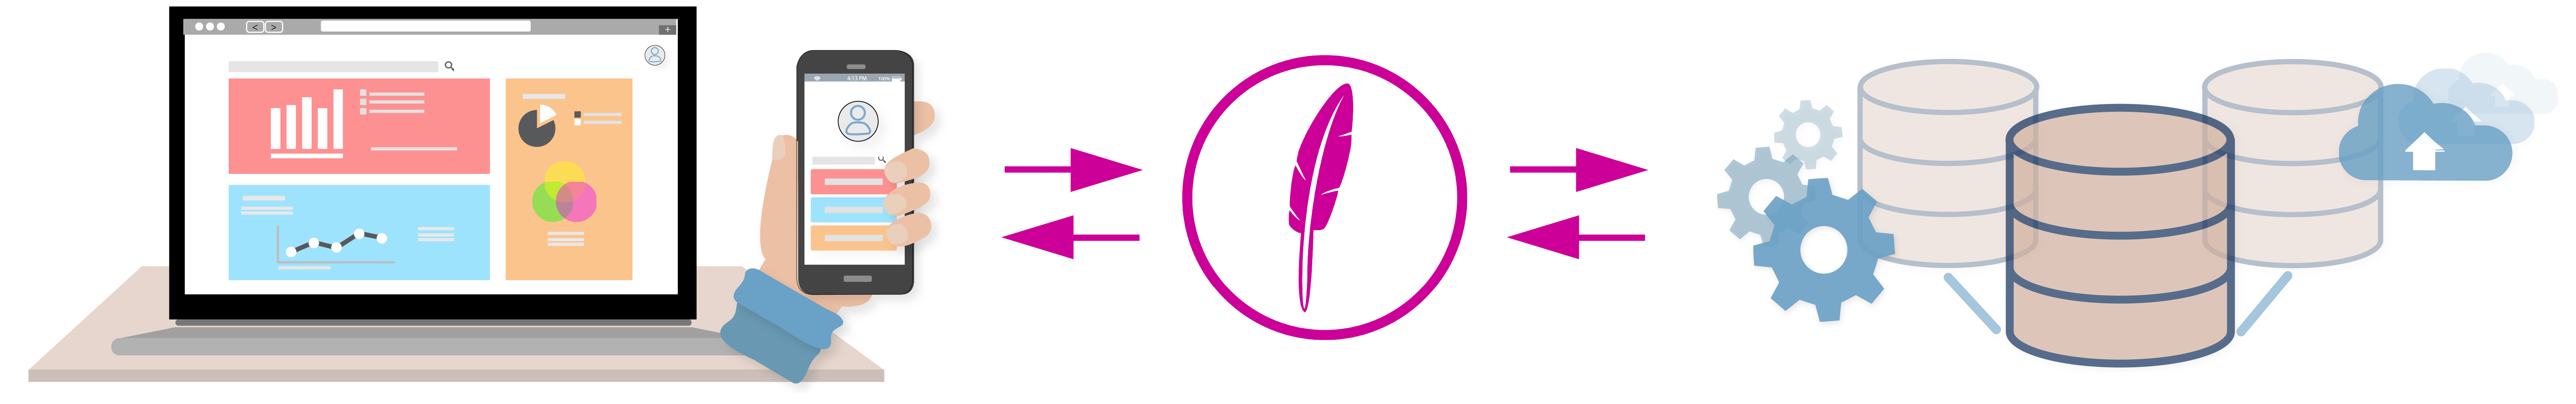
\includegraphics[width=15cm]{feathersuse.png}
	\end{center}
	\vs[1]
	\begin{wrapfigure}{T}{0.3\textwidth}
		\centering
		\vspace{-30pt}
		
\includegraphics[width=0.25\textwidth]{ffmpeg.png}
		\vspace{-80pt}
	\end{wrapfigure}
	\vs
	\textbf{\Large ffmpeg}
	\vs
	FFmpeg is a free and open-source software project consisting of a large suite of libraries and programs for handling video, audio, and other multimedia files and streams. At its core is the FFmpeg program itself, designed for command-line-based processing of video and audio files, and widely used for format transcoding, basic editing (trimming and concatenation), video scaling, video post-production effects, and standards compliance (SMPTE, ITU).
	
	FFmpeg includes libavcodec, an audio/video codec library used by many commercial and free software products, libavformat (Lavf), an audio/video container mux and demux library, and the core ffmpeg command-line program for transcoding multimedia files.
	
	FFmpeg is part of the workflow of hundreds of other software projects, and its libraries are a core part of software media players such as VLC, and has been included in core processing for YouTube and iTunes. Codecs for the encoding and/or decoding of most audio and video file formats is included, making it highly useful for the transcoding of common and uncommon media files into a single common format.
	
	The name of the project is inspired by the MPEG video standards group, together with "FF" for "fast forward". The logo uses a zigzag pattern that shows how MPEG video codecs handle entropy encoding.
	\subsection{Client Side Technology}
	\begin{wrapfigure}{T}{0.2\textwidth}
		\centering
		\vspace{-30pt}
		
\includegraphics[width=0.20\textwidth]{vue.png}
		\vspace{-40pt}
	\end{wrapfigure}
	\vs
	\textbf{\Large vue.js}
	\vs
	Vue (pronounced like view) is a progressive framework for building user interfaces. Unlike other monolithic frameworks, Vue is designed from the ground up to be incrementally adoptable. The core library is focused on the view layer only, and is easy to pick up and integrate with other libraries or existing projects. On the other hand, Vue is also perfectly capable of powering sophisticated Single-Page Applications when used in combination with modern tooling and supporting libraries.
	\vs[1.5]
	\begin{wrapfigure}{T}{0.2\textwidth}
		\centering
		\vspace{-40pt}
		
\includegraphics[width=0.10\textwidth]{vuetify.png}
		\vspace{-10pt}
	\end{wrapfigure}
	\vs
	\textbf{\Large vuetify.js}
	\vs
	Vuetify is the 1 component library for Vue.js and has been in active development since 2016. The goal of the project is to provide users with everything that is needed to build rich and engaging web applications using the Material Design specification. It accomplishes that with a consistent update cycle, Long-term Support (LTS) for previous versions, responsive community engagement, a vast ecosystem of resources and a dedication to quality components.
		\vs[1.5]
	\begin{wrapfigure}{T}{0.2\textwidth}
		\centering
		\vspace{-30pt}
		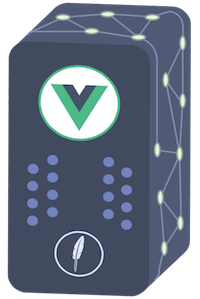
\includegraphics[width=0.10\textwidth]{vuex.png}
		\vspace{-10pt}
	\end{wrapfigure}
	\vs
	\textbf{\Large feathers-vuex}
	\vs
	Feathers-Vuex is a first class integration of FeathersJS and Vuex. It implements many Redux best practices under the hood, eliminates a lot of boilerplate code with flexible data modeling, and still allows you to easily customize the Vuex store.
	\vs[1.5]
	\begin{wrapfigure}{T}{0.2\textwidth}
		\centering
		\vspace{-20pt}
		
\includegraphics[width=0.15\textwidth]{electron.png}
		\vspace{-10pt}
	\end{wrapfigure}
	\vs
	\textbf{\Large electron.js}
	\vs
	Electron (formerly known as Atom Shell) is an open-source software framework developed and maintained by GitHub. It allows for the development of desktop GUI applications using web technologies: it combines the Chromium rendering engine and the Node.js runtime. Electron is the main GUI framework behind several notable open-source projects including Atom  GitHub Desktop, Light Table, Visual Studio Code, and WordPress Desktop.
	
	Electron applications are composed of multiple processes. There is the \emph{browser} process and several \emph{renderer} processes. The browser process runs the application logic, and can then launch multiple renderer processes, rendering the windows that appear on a user's screen rendering HTML and CSS.
	
	Both the browser and renderer processes can run with Node.js integration if enabled.
	
	Most of Electron's APIs are written in C++ or Objective-C and then exposed directly to the application code through JavaScript bindings.
	\vs[1.5]
	
